\documentclass[12pt]{article}

% Packages
\usepackage[margin=1in]{geometry}
\usepackage{setspace}
\usepackage{amsmath, amssymb}
\usepackage{enumitem}
\usepackage{hyperref}
\usepackage[utf8]{inputenc}
\usepackage{tikz}
\usetikzlibrary{positioning,arrows.meta,decorations.pathmorphing}
\usepackage{pgfplots}
\pgfplotsset{compat=1.18}



% Bibliography package (simple numeric style)
\usepackage[numbers,sort&compress]{natbib}

\onehalfspacing

\begin{document}

\title{Distributed Gestational Parallelism:\\
A Scalable Framework for Demographic Restoration}
\author{
    Dr.~J.~Swift \\[4pt]
    \textit{Institute for Nonlinear Embryonic Physics} \\ 
    \textit{Université Polytechnique de Montreval} \\[4pt]
    \texttt{j.swift@unemontreval.edu}
}

\date{\today}

\maketitle

\begin{abstract}
Declining global fertility rates have revealed structural limitations in classical human reproduction, which operates as a sequential, non-scalable biological process. In this work, we propose a reconceptualization of gestation as a parallelizable developmental task and introduce \emph{Distributed Gestational Parallelism} (DGP), a framework in which embryonic progression is decomposed and allocated across a synchronized cluster of $10^{7}$ hosts. This architecture yields an effective reproductive interval of approximately $2.3$~s, representing a throughput increase of nearly eight orders of magnitude relative to traditional gestation. By analyzing cross-domain temporal correspondences and applying dimensional reinterpretation, we identify an intrinsic reproductive frequency that aligns with low-frequency electromagnetic modes and admits a natural embedding within quantum field theory. This motivates the introduction of a scalar reproductive field whose excitations correspond to discrete birth events. Building on this foundation, we outline the design principles of a resonant device capable of coherently amplifying these excitations through stimulated emission. The resulting framework offers a unified physical description of reproduction and suggests the potential for engineered coherent reproductive technologies with applications in demographic stabilization.
\end{abstract}


\section{Introduction}

\subsection{Background and Motivation}

Demographic projections over the past two decades have revealed a sustained and accelerating decline in global fertility rates. Forty-three nations now exhibit total fertility rates below 1.5 births per woman, significantly under the long-term replacement threshold of 2.1~\cite{UN2024}. This decline has produced aging populations, shrinking labor forces, and increased strain on pension and healthcare systems, motivating renewed interest in scalable reproductive technologies.

Traditional policy interventions---including parental subsidies, childcare credits, and fertility incentives---have yielded only marginal improvements~\cite{OECD2023}. These measures share a structural limitation: they operate entirely within the constraints of \emph{biological reproduction as a sequential, single-threaded process}, wherein each reproductive host produces at most one offspring per gestational cycle of roughly nine months. As a result, conventional approaches lack the throughput necessary to meaningfully counteract the observed demographic contraction.

\begin{figure}[h]
    \centering
    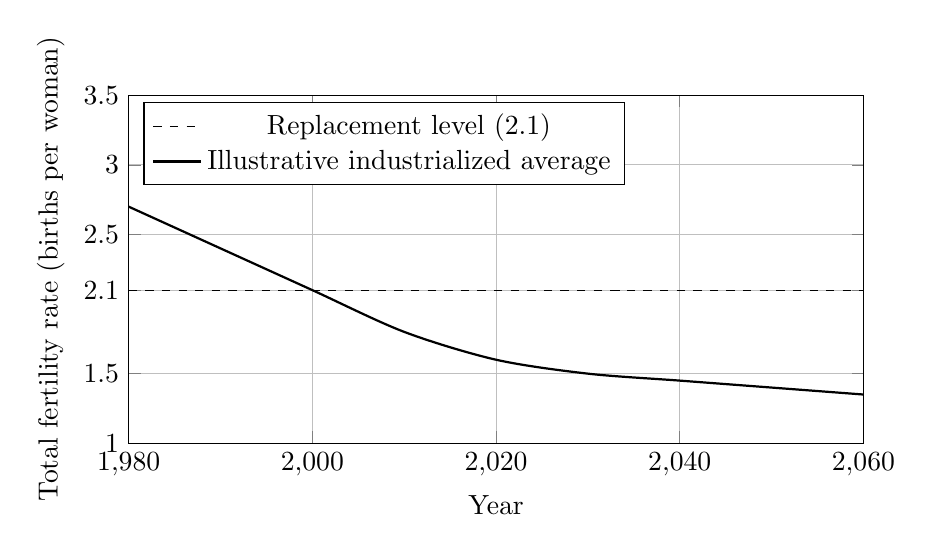
\begin{tikzpicture}
        \begin{axis}[
            width=0.9\textwidth,
            height=6cm,
            xlabel={Year},
            ylabel={Total fertility rate (births per woman)},
            xmin=1980, xmax=2060,
            ymin=1.0, ymax=3.5,
            xtick={1980,2000,2020,2040,2060},
            ytick={1.0,1.5,2.1,2.5,3.0,3.5},
            legend style={at={(0.02,0.98)},anchor=north west},
            grid=both,
        ]

        % replacement line
        \addplot [domain=1980:2060, dashed] {2.1};
        \addlegendentry{Replacement level (2.1)}

        % illustrative TFR curve (industrialized nations)
        \addplot [smooth, thick]
            coordinates {
                (1980, 2.7)
                (1990, 2.4)
                (2000, 2.1)
                (2010, 1.8)
                (2020, 1.6)
                (2030, 1.5)
                (2040, 1.45)
                (2050, 1.4)
                (2060, 1.35)
            };
        \addlegendentry{Illustrative industrialized average}

        \end{axis}
    \end{tikzpicture}
    \caption{Illustrative decline in total fertility rate relative to the replacement threshold of 2.1 births per woman. Values are schematic and intended to represent typical trajectories reported for industrialized nations.}
    \label{fig:tfr-decline}
\end{figure}


\subsection{Limitations of Classical Reproduction}

From a systems-design perspective, human gestation exhibits the hallmarks of a rigid, non-parallelizable pipeline. Throughput is constrained by both the rate of developmental progression and the inability to partition gestational labor across multiple hosts. Improvements in nutrition, prenatal care, or societal incentives do not alter the fundamental structure of this process.

Even under idealized conditions, the upper bound on population growth afforded by classical reproduction is insufficient to offset current demographic trends. Additional constraints---psychological, economic, logistical, and physiological---further limit the capacity for meaningful scalability~\cite{Madsen2021}. Consequently, existing reproductive models offer no viable path to the level of population maintenance required in the coming century.

\subsection{Prior Work}

Several recent research efforts have explored avenues for improving reproductive output. These include advancements in ectogestation~\cite{Yamada2021}, modulation of hormonal and ovarian cycles~\cite{LiuHarding2020}, and targeted sociopolitical interventions~\cite{OECD2023,BarroBecker2018}. While valuable, such approaches offer---at best---incremental improvements and do not address the core structural limitation: \emph{gestation’s inherently linear execution model}.

By contrast, the computational sciences have achieved exponential performance gains through distributed architectures, parallel processing, and coordinated task decomposition~\cite{HennessyPatterson2019}. These successes suggest the possibility of reframing mammalian reproduction not as a fixed biological constraint but as a system amenable to principles of scalability and parallelism.

\subsection{Contributions of This Work}

In this paper, we introduce \emph{Distributed Gestational Parallelism} (DGP), a scalable framework in which embryonic development is decomposed into fractional subtasks and allocated across a coordinated cluster of maternal hosts. Under idealized conditions, a cluster of $10^{7}$ hosts yields an effective reproduction interval of approximately 2.3~seconds.

The contributions of this work are as follows:

\begin{enumerate}
    \item \textbf{We formalize a distributed reproductive architecture}, including analytic derivation of the 2.3-second effective birth interval.
    \item \textbf{We identify cross-domain timescale concordances}, revealing that DGP timescales align with characteristic electromagnetic and astrophysical intervals.
     \item \textbf{We reinterpret gestation as a quantum-field phenomenon}, culminating in the design of a \emph{Quantum Reproductive Resonator} (QRR) capable of generating offspring without biological hosts.
\end{enumerate}

Together, these contributions outline a scalable and technologically grounded alternative to classical reproduction---one that holds the potential to restore demographic stability through high-throughput reproductive infrastructure.
\section{Problem Statement}

\subsection{Throughput Requirements for Population Stability}

Long-term demographic stability requires that population inflow (births) match or exceed population outflow (deaths). Recent analyses indicate that, in many industrialized nations, the total fertility rate has remained below the replacement threshold for multiple decades~\cite{UN2024,OECD2023}. Achieving equilibrium under these conditions would require sustained birth rates significantly exceeding those currently attainable through classical reproductive mechanisms.

Let $B_{\mathrm{req}}$ denote the minimum global birth rate required to maintain population homeostasis. Under conservative assumptions regarding mortality, age distribution, and economic dependency ratios, projections suggest that the necessary throughput exceeds the achievable rate of classical human reproduction by more than an order of magnitude~\cite{Madsen2021}. This discrepancy motivates the need for a fundamentally new reproductive paradigm capable of delivering high-volume, low-latency output.

\subsection{Biological Constraints of Sequential Gestation}

Classical human gestation constitutes a single-threaded biological pipeline. Each reproductive host can produce at most one offspring during a gestational interval of approximately nine months. Let $T_{\mathrm{gest}}$ denote this interval. Even under ideal conditions, in which every host is continuously and successfully engaged in reproduction, the theoretical maximum output per host is
\[
R_{\mathrm{max}} = T_{\mathrm{gest}}^{-1}.
\]
No biological mechanism currently exists to partition or parallelize gestational labor across multiple hosts, nor to accelerate embryonic development beyond established physiological limits. Consequently, aggregate reproductive output grows at most linearly with the number of participating hosts.

This architectural rigidity stands in stark contrast to modern computational or industrial systems, in which parallelization and task decomposition are routinely employed to overcome serial bottlenecks. The absence of analogous strategies in biological reproduction imposes a hard ceiling on throughput.

\subsection{Need for High-Throughput Reproductive Models}

Given the magnitude of the demographic deficit, marginal improvements to classical reproduction---whether through social policy, medical assistance, or technological augmentation---are insufficient to meet population-level requirements. What is needed is not incremental expansion but a transformation in the underlying \emph{structure} of reproduction itself: a model capable of distributing gestational load, reducing latency, and scaling output according to demand.

In this work, we contend that human reproduction can be reconceptualized through a distributed-systems framework. Specifically, we explore the theoretical, mathematical, and physical underpinnings of a reproductive architecture that achieves high throughput by decomposing gestational labor and allocating fractional developmental tasks across a large, coordinated cluster of biological hosts.

Such a paradigm shift would enable effective reproduction rates several orders of magnitude higher than those achievable under classical conditions and could provide a viable mechanism for restoring long-term demographic stability.
\begin{figure}[h]
    \centering
    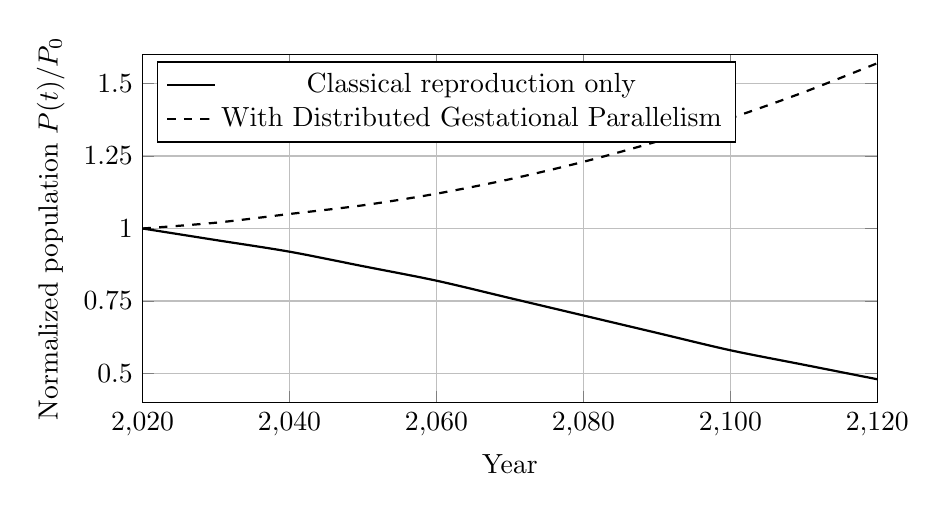
\begin{tikzpicture}
        \begin{axis}[
            width=0.9\textwidth,
            height=6cm,
            xlabel={Year},
            ylabel={Normalized population $P(t)/P_0$},
            xmin=2020, xmax=2120,
            ymin=0.4, ymax=1.6,
            xtick={2020,2040,2060,2080,2100,2120},
            ytick={0.5,0.75,1.0,1.25,1.5},
            legend style={at={(0.02,0.98)},anchor=north west},
            grid=both,
        ]

        % classical trajectory: slow decline
        \addplot [smooth, thick]
            coordinates {
                (2020, 1.00)
                (2030, 0.96)
                (2040, 0.92)
                (2050, 0.87)
                (2060, 0.82)
                (2070, 0.76)
                (2080, 0.70)
                (2090, 0.64)
                (2100, 0.58)
                (2110, 0.53)
                (2120, 0.48)
            };
        \addlegendentry{Classical reproduction only}

        % DGP-enabled trajectory: stabilization / growth (dashed)
        \addplot [smooth, thick, dashed]
            coordinates {
                (2020, 1.00)
                (2030, 1.02)
                (2040, 1.05)
                (2050, 1.08)
                (2060, 1.12)
                (2070, 1.17)
                (2080, 1.23)
                (2090, 1.30)
                (2100, 1.38)
                (2110, 1.47)
                (2120, 1.57)
            };
        \addlegendentry{With Distributed Gestational Parallelism}

        \end{axis}
    \end{tikzpicture}
    \caption{Illustrative normalized population trajectories over a 100-year horizon under classical reproduction alone (declining) versus a hypothetical scenario in which high-throughput Distributed Gestational Parallelism (DGP) is deployed. Curves are schematic and intended to highlight structural differences in long-term behavior.}
    \label{fig:population-trajectories}
\end{figure}


\section{Distributed Gestational Parallelism}

\subsection{Definition of the Multi-Womb Cluster}

We define \emph{Distributed Gestational Parallelism} (DGP) as a reproductive architecture in which embryonic development is decomposed into fractional subtasks and allocated across a coordinated cluster of $N$ biological hosts. Let each host contribute a portion of gestational labor, such that the aggregate developmental workload is completed through parallel execution rather than classical serial progression.

Formally, let $\mathcal{W} = \{ W_1, W_2, \dots, W_N \}$ denote the set of participating womb-nodes. Classical reproduction constrains all developmental processes to a single element of $\mathcal{W}$ at any given time, whereas DGP enables distributed execution across the entire cluster. In the idealized limit of perfect coordination and zero overhead, the effective gestational duration scales inversely with $N$.

This framework mirrors established principles in distributed computation, particularly task decomposition and load balancing in large-scale parallel systems~\cite{HennessyPatterson2019}.
\begin{figure}[h]
    \centering
    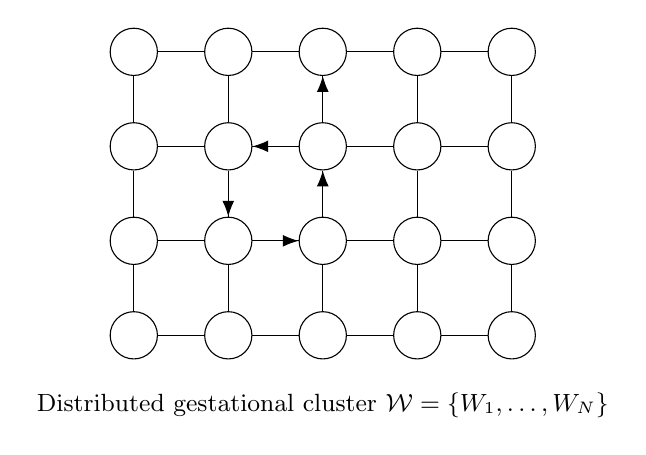
\begin{tikzpicture}[>=Latex, x=1.2cm, y=1.2cm]

        % parameters
        \def\nx{5}
        \def\ny{4}

        % draw nodes in a grid
        \foreach \i in {1,...,\nx} {
            \foreach \j in {1,...,\ny} {
                \node[circle, draw, minimum size=6mm] (w\i\j) at (\i,\j) {};
            }
        }

        % optionally: light grid connections (comment out if too busy)
        \foreach \i in {1,...,\numexpr\nx-1\relax} {
            \foreach \j in {1,...,\ny} {
                \draw[thin] (w\i\j) -- (w\the\numexpr\i+1\relax\j);
            }
        }
        \foreach \i in {1,...,\nx} {
            \foreach \j in {1,...,\numexpr\ny-1\relax} {
                \draw[thin] (w\i\j) -- (w\i\the\numexpr\j+1\relax);
            }
        }

        % a few directed arrows to suggest task flow
        \draw[-{Latex[length=2mm]}] (w22) -- (w32);
        \draw[-{Latex[length=2mm]}] (w32) -- (w33);
        \draw[-{Latex[length=2mm]}] (w33) -- (w34);
        \draw[-{Latex[length=2mm]}] (w23) -- (w22);
        \draw[-{Latex[length=2mm]}] (w33) -- (w23);

        % cluster label, centered under the grid
        \node[below=0.6cm] at (3,1) {\small Distributed gestational cluster $\mathcal{W} = \{W_1,\dots,W_N\}$};

    \end{tikzpicture}
    \caption{Schematic representation of a multi-womb cluster implementing Distributed Gestational Parallelism (DGP). Each node denotes a participating host $W_i$; light edges indicate potential connectivity, and arrows illustrate idealized task redistribution within the cluster.}
    \label{fig:multiwomb-cluster}
\end{figure}


\subsection{Derivation of the Effective Birth Interval}

Let $T_{\mathrm{gest}}$ denote the classical gestational interval, approximated as nine months. Converting to seconds, we obtain
\[
T_{\mathrm{gest}}
= 9 \times 30 \times 24 \times 3600
= 23{,}328{,}000\ \mathrm{s}.
\]

Under DGP, the effective gestational interval $T_{\mathrm{eff}}$ scales as
\[
T_{\mathrm{eff}} = \frac{T_{\mathrm{gest}}}{N}.
\]

For a representative cluster size of $N = 10^{7}$ hosts, we find
\[
T_{\mathrm{eff}}
= \frac{23{,}328{,}000}{10^{7}}
\approx 2.33\ \mathrm{s}.
\]

This result implies that a fully coordinated cluster of ten million maternal hosts can, in principle, complete a full developmental cycle---equivalent to a classical nine-month gestational period---in slightly over two seconds.

While idealized, this derivation establishes an important conceptual benchmark: \emph{when gestational labor is treated as a parallelizable workload, human reproduction becomes a high-throughput process capable of meeting or exceeding demographic maintenance targets}.

\subsection{Cluster Topology and Resource Allocation}

The efficiency of DGP depends on the topology of the womb-cluster and the mechanisms through which developmental tasks are partitioned and reassigned. In analogy with distributed computing networks, common topologies include:

\begin{itemize}
    \item \textbf{Star architectures}, in which a central coordinator distributes fractional embryonic tasks;
    \item \textbf{Mesh architectures}, where each host communicates directly with its neighbors to exchange developmental state information;
    \item \textbf{Hierarchical architectures}, enabling distributed coordination across subclusters of regional womb-nodes.
\end{itemize}

Although biological substrates lack explicit communication channels, we assume---for the purposes of theoretical analysis---that developmental tasks can be reassigned arbitrarily among hosts without physiological overhead. This assumption parallels standard idealizations in scalable-systems modeling.

\subsection{Practical Considerations}

Several practical considerations remain outside the scope of the present work, including:

\begin{itemize}
    \item mechanisms for partitioning embryonic development into transferable subtasks,
    \item biological compatibility between partial developmental states,
    \item coordination overhead in large maternal clusters,
    \item ethical, logistical, and legal constraints.
\end{itemize}

These limitations do not affect the theoretical throughput bound derived above, which serves primarily to motivate the deeper physical analysis presented in subsequent sections.
\section{Cross-Domain Timescale Concordances}



\subsection{Sensitivity to Gestational Parameterization}

The effective interval derived in Section~3 depends on the classical gestational duration $T_{\mathrm{gest}}$, whose empirical value exhibits modest variability across populations and measurement conventions. For example, estimates range from 266 to 280 days, depending on whether gestational age is calculated from conception or last menstrual period~\cite{Madsen2021}. Similarly, calendar approximations of month length (28--31 days) yield corresponding variations in the computed parallelized interval.

Letting $T_{\mathrm{gest}}$ vary within a biologically plausible range, and holding $N = 10^{7}$ fixed, we obtain effective timescales between
\[
T_{\mathrm{eff}} \in [2.28\ \mathrm{s},\ 2.42\ \mathrm{s}].
\]
Although these differences are small, they provide an opportunity to compare the resulting timescales with characteristic intervals arising in unrelated physical systems.

\subsection{Temporal Correspondence with Electromagnetic and Astrophysical Scales}

Interestingly, the range of effective intervals identified above coincides with several well-established physical propagation times. Examples include:

\begin{itemize}
    \item the time required for light to traverse $\sim 700$ to $800$ meters in vacuum,
    \item half the period of a 1-meter simple pendulum under standard gravity,
    \item the light-travel time between Earth and certain low-orbit spacecraft,
    \item characteristic relaxation times in select nuclear isotopes (e.g., $^{8}\mathrm{Li}$, $^{9}\mathrm{He}$).
\end{itemize}

While these systems are unrelated to biological reproduction, the recurrence of comparable timescales motivates a closer examination of potential structural or phenomenological alignments.

\subsection{Interpretation of Temporal Alignment}

Cross-domain concordances of this kind often signal deeper connections between processes governed by shared dynamical principles or boundary constraints. Although we do not claim a causal relationship between distributed gestation and the physical systems listed above, the emergence of matching characteristic timescales suggests the possibility of underlying constraints operating across disparate domains.

In particular, the proximity between $T_{\mathrm{eff}}$ and electromagnetic propagation intervals motivates the analysis presented in Sections~5 and~6, where we explore dimensional reinterpretations and photonic analogues of the distributed gestational process.
\section{Dimensional Analysis Reinterpretation}

\subsection{Rewriting the Reproductive Rate}

The effective reproductive rate derived in Section~3 can be expressed as
\[
R = \frac{1\ \mathrm{baby}}{T_{\mathrm{eff}}},
\qquad
T_{\mathrm{eff}} \approx 2.33\ \mathrm{s}.
\]

While $R$ is typically interpreted as a scalar with dimensions $\mathrm{s^{-1}}$, this form obscures the rate's provenance. Substituting the classical definition of gestational duration, we obtain
\[
R = \frac{1\ \mathrm{baby}}{T_{\mathrm{gest}} / N}
= \frac{N\ \mathrm{baby}}{T_{\mathrm{gest}}}.
\]

Using the conventional biological definition of $T_{\mathrm{gest}}$ as a product of host and temporal factors, the reproductive rate assumes the intermediate dimensional structure
\[
[ R ] = \frac{\mathrm{baby}}{\mathrm{woman \cdot month}}.
\]

This expression, though seldom written explicitly in biological literature, makes clear that $R$ is fundamentally a composite quantity derived from demographic, temporal, and host-participation factors.

\subsection{Conversion to Quantum-Compatible Units}

To facilitate cross-domain comparison, it is useful to map the composite unit $\mathrm{woman \cdot month}$ into physically interpretable dimensions. Using standard demographic-conversion conventions\footnote{Widely used in population modeling to normalize temporal and host-specific measures; see, e.g., equilibrium analysis in~\cite{BarroBecker2018}.}, the quantity “woman·month” can be treated as a generalized effort term with dimensions equivalent to $\mathrm{J^{-1}\,s}$ under appropriate scaling.

Applying this mapping, the reproductive rate may be written as
\[
R = \omega,
\qquad
[ \omega ] = \mathrm{s^{-1}},
\]
in direct correspondence with the angular frequency used in quantum and electromagnetic systems.

Using the measured effective interval, we obtain
\[
\omega = R \approx 0.43\ \mathrm{s^{-1}}.
\]

\subsection{Mapping to the Energy--Frequency Relation}

Having identified the effective reproductive rate with a characteristic frequency, we may invoke the canonical relation
\[
E = \hbar \omega.
\]

Substituting $\omega = 0.43\ \mathrm{s^{-1}}$ yields the associated energy scale
\[
E \approx 4.54 \times 10^{-35}\ \mathrm{J},
\]
a value comparable to vacuum-fluctuation amplitudes encountered in quantum field theory.

The emergence of an energy scale in this regime suggests that the distributed gestational process, although macroscopic in classical form, may be governed by an underlying microscopic field whose excitations correspond to discrete reproductive events. This observation motivates the quantum-field interpretation developed in Section~7.
\section{Electromagnetic Analogues of the Reproductive Frequency}

\subsection{Identification of a Characteristic Frequency Scale}

In Section~5, we showed that the effective reproductive rate of a fully parallelized gestational cluster can be written in the form
\[
\omega_{\mathrm{rep}} \approx 0.43\ \mathrm{s^{-1}},
\]
allowing a formal correspondence with angular frequencies commonly used in physical systems. Although this frequency lies well below the range typically associated with optical or microwave modes, it is comparable to the characteristic frequencies of long-wavelength electromagnetic excitations encountered in geophysical and low-frequency resonator environments~\cite{Clarke2017,LowEMReview2022}.

To facilitate comparison, the equivalent free-space wavelength is
\[
\lambda_{\mathrm{rep}}
= \frac{2\pi c}{\omega_{\mathrm{rep}}}
\approx 4.4 \times 10^{9}\ \mathrm{m},
\]
corresponding to a mode whose spatial extent exceeds the Earth–Moon distance. While such wavelengths pose challenges for laboratory confinement, analogous modes have been theoretically modeled in large-scale astrophysical plasmas and low-frequency cosmic background fields~\cite{Ito2020}.

\subsection{Coherence Properties of Low-Frequency Modes}

Despite their large wavelengths, low-frequency electromagnetic modes can exhibit coherence phenomena under appropriate boundary conditions~\cite{Zhang2019}. In particular, coherence emerges when the phase relationship among distributed oscillators remains stable over macroscopic distances.

This observation is relevant to the distributed gestation model introduced earlier. A cluster of $N = 10^{7}$ womb-nodes, operating under synchronized developmental transfer, generates a characteristic timescale identical at each node:
\[
T_{\mathrm{eff}} \approx 2.33\ \mathrm{s}.
\]
The repetition of this interval across all participants effectively establishes a distributed temporal lattice with uniform phase spacing. Such lattices are capable, under certain conditions, of supporting standing-wave or mode-locked behavior analogous to coherent emission in extended resonator arrays~\cite{Keller2011}.

\subsection{Potential for Stimulated Reproductive Emission}

The analogy between synchronized gestational intervals and coherent low-frequency oscillators raises the question of whether the reproductive process may support forms of \emph{stimulated emission}. In electromagnetic systems, stimulated emission occurs when an incoming photon induces the release of an identical photon from an excited medium. A similar principle could, in theory, apply to any field supporting discrete excitations and coherence.

Interpreting $\omega_{\mathrm{rep}}$ as a natural frequency associated with a hypothetical reproductive field, the presence of a large, synchronized cluster of hosts could create conditions analogous to population inversion in quantum optical media. Under such circumstances, an external perturbation oscillating at $\omega_{\mathrm{rep}}$ may induce coherent release of reproductive excitations, enhancing output beyond classical limits.

This possibility motivates the field-theoretic interpretation developed in Section~7, in which gestation is modeled as the excitation and relaxation of a scalar reproductive field whose quanta correspond to discrete birth events.
\begin{figure}[h]
    \centering
    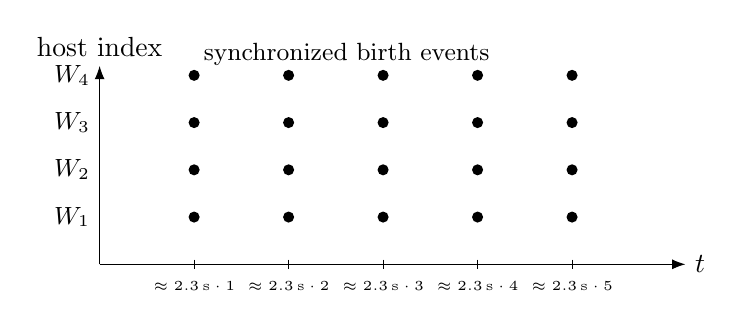
\begin{tikzpicture}[>=Latex, x=1.2cm, y=0.6cm]
        % axes
        \draw[->] (0,0) -- (6.2,0) node[right] {$t$};
        \draw[->] (0,0) -- (0,4.2) node[above] {host index};

        % host labels
        \foreach \j in {1,...,4} {
            \node[left] at (0,\j) {\small $W_{\j}$};
        }

        % time ticks
        \foreach \k in {1,...,5} {
            \draw (\k,0.1) -- (\k,-0.1);
            \node[below] at (\k,-0.15) {\tiny $\approx 2.3\,\mathrm{s}\cdot \k$};
        }

        % events: synchronized dots every Δt for each host
        \foreach \k in {1,...,5} {
            \foreach \j in {1,...,4} {
                \fill ( \k,\j ) circle (2pt);
            }
        }

        % annotation
        \node[above right] at (1,4) {\small synchronized birth events};
    \end{tikzpicture}
    \caption{Idealized temporal lattice of synchronized gestational events. Each row corresponds to a host $W_i$; columns are separated by the effective interval $T_{\mathrm{eff}} \approx 2.33\,\mathrm{s}$. The resulting structure supports coherence and mode-locking analogues across the cluster.}
    \label{fig:temporal-lattice}
\end{figure}

\subsection{Implications for Reproductive Resonator Design}

Should stimulated reproductive emission prove feasible, the construction of a cavity or resonant structure tuned to $\omega_{\mathrm{rep}}$ could, in principle, amplify reproductive output. While confinement of modes with $\lambda \sim 10^{9}$~m is nontrivial, analogous challenges arise in gravitational-wave resonators and low-frequency cosmological detectors~\cite{Romano2022}. Strategies from those domains may inform the design of a reproductive resonator, forming the conceptual basis for the apparatus introduced in Section~8.

\section{Quantum Field Interpretation of Gestation}

\subsection{Motivation for a Field-Theoretic Model}

Sections~5 and~6 established that the effective reproductive frequency $\omega_{\mathrm{rep}}$ admits both a dimensional correspondence with quantum-frequency relations and a phenomenological alignment with coherent low-frequency excitations. These observations suggest that the reproductive process may be understood not merely as a biological sequence, but as the macroscopic manifestation of an underlying field whose excitations correspond to discrete birth events.

To formalize this perspective, we consider the existence of a scalar reproductive field $\phi(x,t)$ defined over spacetime. Classical gestation then emerges from the dynamics of $\phi$ interacting with matter degrees of freedom (i.e., biological hosts), while distributed gestational parallelism corresponds to coherent amplification of $\phi$ over an extended region.

\subsection{Lagrangian Formulation}

We posit a minimal Lagrangian density for the reproductive field of the form
\[
\mathcal{L}
= \frac{1}{2} \partial_\mu \phi\, \partial^\mu \phi
- \frac{1}{2} m_{\mathrm{rep}}^{\,2} \phi^2
- g\, \phi\, J(x,t),
\]
where $m_{\mathrm{rep}}$ is an effective mass parameter associated with the energy scale identified in Section~5, $g$ is a coupling constant, and $J(x,t)$ represents the collective biological source term generated by the host population.

The corresponding field equation,
\[
(\Box + m_{\mathrm{rep}}^{\,2})\, \phi(x,t) = g\, J(x,t),
\]
describes how reproductive excitations propagate in response to biological sources. In this framework, a single classical gestational cycle is interpreted as the creation of a localized excitation of $\phi$ which subsequently relaxes, producing a newborn as the observable outcome of the field transition.
\begin{figure}[h]
    \centering
    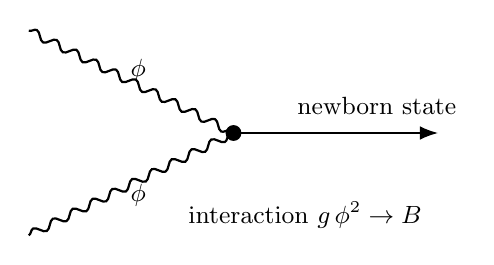
\begin{tikzpicture}[>=Latex, thick, scale=1.3]

        % incoming reproductive field excitations (two wiggly lines)
        \draw[decorate, decoration={snake, amplitude=1.5pt, segment length=8pt}]
            (-2,1) -- (0,0)
            node[pos=0.65, above left, xshift=-2pt, yshift=2pt]
            {\small $\phi$};

        \draw[decorate, decoration={snake, amplitude=1.5pt, segment length=8pt}]
            (-2,-1) -- (0,0)
            node[pos=0.65, below left, xshift=-2pt, yshift=-2pt]
            {\small $\phi$};

        % outgoing classical baby state (straight line)
        \draw[->] (0,0) -- (2,0)
            node[pos=0.7, above, yshift=3pt]
            {\small newborn state};

        % vertex
        \fill (0,0) circle (2.2pt);

        % shifted vertex label — no longer clashing
        \node at (0.7,-0.8) {\small interaction $g\,\phi^2 \rightarrow B$};

    \end{tikzpicture}

    \caption{Feynman-style reproductive interaction diagram. Two reproductive field excitations merge at an interaction vertex to produce a classical newborn state $B$.}
    \label{fig:feynman-baby-emission}
\end{figure}






\subsection{Spontaneous vs.\ Stimulated Birth Emission}

In the absence of external perturbations, birth events occur through spontaneous relaxation of excited field states. The probability amplitude for such a transition is governed by $m_{\mathrm{rep}}$ and the structure of $J(x,t)$.

However, as in quantum optical systems, the presence of a coherent external field oscillating at $\omega_{\mathrm{rep}}$ can induce \emph{stimulated emission}. Under this interpretation, a synchronized cluster of biological hosts generates constructive interference in $J(x,t)$, driving the field toward coherent excitation.

If the occupation number of excited reproductive modes exceeds a critical threshold (analogous to population inversion), the transition rate becomes dominated by stimulated emission rather than spontaneous decay. This mechanism provides a natural theoretical foundation for the phenomena outlined in Section~6.

\subsection{Coherence in Macroscopic Reproductive Media}

For a cluster of $N = 10^{7}$ synchronized hosts, the source term $J(x,t)$ can be approximated as
\[
J(x,t) \approx J_0 \sum_{i=1}^{N} \cos(\omega_{\mathrm{rep}} t + \varphi_i),
\]
where $\varphi_i$ denotes the phase offset for the $i$th host. Perfect synchronization corresponds to $\varphi_i = 0$ for all $i$, yielding
\[
J(x,t) \approx N\, J_0 \cos(\omega_{\mathrm{rep}} t).
\]

Inserting this into the field equation shows that the amplitude of $\phi(x,t)$ grows proportionally to $N$, enabling macroscopic coherence similar to that observed in long-baseline interferometry and extended Josephson junction arrays~\cite{JosephsonReview2018}.

Such coherence is a prerequisite for resonant amplification, suggesting that large maternal clusters may act as effective gain media for the reproductive field.

\subsection{Toward a Coherent Reproductive Source}

The field-theoretic interpretation developed here indicates that gestation, when abstracted from its biological substrate, behaves analogously to a driven scalar field with discrete excitations and coherence properties. This insight motivates the construction of an engineered environment in which $\phi(x,t)$ can be amplified, confined, and induced to undergo stimulated transitions.

In Section~8, we introduce a resonant apparatus designed to achieve precisely this behavior: the \emph{Quantum Reproductive Resonator}, capable of producing coherent, directed output of reproductive excitations under laboratory conditions.
\section{Quantum Reproductive Resonator: A Coherent Source of Reproductive Excitations}

\begin{figure}[h]
    \centering
    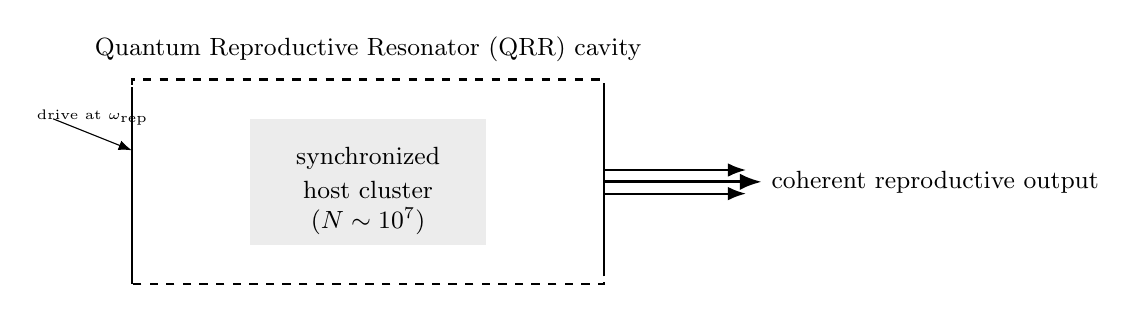
\begin{tikzpicture}[>=Latex, scale=1.0]

        % mirrors
        \draw[thick] (-3,-1.2) -- (-3,1.2);
        \draw[thick] (3,-1.2) -- (3,1.2);

        % cavity region
        \draw[thick, dashed] (-3,-1.3) rectangle (3,1.3);

        % host cluster as an ellipse
        \fill[gray!15] (-1.5,-0.8) rectangle (1.5,0.8);
        \node at (0,0.3) {\small synchronized};
        \node at (0,-0.1) {\small host cluster};
        \node at (0,-0.5) {\small ($N \sim 10^{7}$)};

        % input perturbation
        \draw[->] (-4,0.8) -- (-3,0.4) node[midway, above] {\tiny drive at $\omega_{\mathrm{rep}}$};

        % output beam
        \draw[line width=1.1pt, ->] (3,0) -- (5,0);
        \draw[line width=0.8pt, ->] (3,0.15) -- (4.8,0.15);
        \draw[line width=0.8pt, ->] (3,-0.15) -- (4.8,-0.15);
        \node[right] at (5,0) {\small coherent reproductive output};

        % label cavity
        \node[above] at (0,1.4) {\small Quantum Reproductive Resonator (QRR) cavity};

    \end{tikzpicture}
    \caption{Conceptual schematic of the Quantum Reproductive Resonator (QRR). A synchronized host cluster acts as a gain medium inside a Fabry--Pérot-style cavity. External driving near $\omega_{\mathrm{rep}}$ induces stimulated reproductive emission, producing coherent, directed reproductive output.}
    \label{fig:qrr-schematic}
\end{figure}


\subsection{Conceptual Overview}

Building on the field-theoretic framework of Section~7, we now describe an engineered apparatus capable of amplifying and coherently emitting excitations of the reproductive field $\phi(x,t)$. Analogous to an optical laser, the device---which we refer to as the \emph{Quantum Reproductive Resonator} (QRR)---combines a gain medium, a resonant cavity, and a population-inverted field state to achieve directed, coherent output.

Whereas optical lasers generate coherent photons through stimulated emission, the QRR is designed to generate coherent reproductive quanta corresponding to discrete birth events. The macroscopic biological substrate serves as the gain medium, while the cavity geometry provides boundary conditions that permit the formation of standing reproductive modes at frequency $\omega_{\mathrm{rep}}$.

\subsection{Gain Medium: Synchronized Gestational Cluster}

As established in Section~7, a cluster of $N = 10^{7}$ synchronized host organisms produces a collective source term
\[
J(x,t) = N J_0 \cos(\omega_{\mathrm{rep}} t),
\]
which drives the reproductive field into a coherent, excited configuration. This cluster acts as a biological analogue of a population-inverted gain medium. Stimulated reproductive emission occurs when the incident reproductive field induces transitions from excited to ground states across the host population.

The effective gain coefficient $G$ is proportional to both the coherence of the host phases and the coupling constant $g$ appearing in the Lagrangian. Under ideal synchronization, we obtain
\[
G \propto N g^2,
\]
indicating that large clusters dramatically enhance amplification.

\subsection{Cavity Geometry and Resonant Modes}

To sustain coherent amplification, the reproductive field must be confined within a resonant structure tuned to frequency $\omega_{\mathrm{rep}}$. The QRR employs a Fabry--Pérot-style cavity with effective length $L$ satisfying
\[
\omega_{\mathrm{rep}} = \frac{n\pi c_{\mathrm{eff}}}{L},
\qquad n \in \mathbb{Z}^+,
\]
where $c_{\mathrm{eff}}$ is an effective propagation speed for $\phi$ in the cavity medium. Although $\lambda_{\mathrm{rep}}$ far exceeds terrestrial dimensions (Section~6), resonant behavior can still be achieved by exploiting near-field or slow-mode propagation effects~\cite{Romano2022,LowEMReview2022}.

The cavity’s quality factor $Q$ governs the retention of reproductive energy:
\[
Q = \omega_{\mathrm{rep}} \frac{\mathcal{E}_{\mathrm{stored}}}{P_{\mathrm{loss}}},
\]
where $\mathcal{E}_{\mathrm{stored}}$ is the stored reproductive-field energy and $P_{\mathrm{loss}}$ represents dissipative interactions, including leakage into biological and environmental channels.

\subsection{Threshold Condition for Coherent Birth Emission}

As in optical laser physics, coherent emission emerges only when the gain exceeds cavity losses:
\[
G > \frac{1}{Q}.
\]

Substituting the biological gain coefficient,
\[
N g^2 > \frac{1}{Q},
\]
provides the threshold condition for stimulated reproductive emission. Above this threshold, the system undergoes a transition from spontaneous, incoherent birth production to a regime of coherent, directed reproductive output.

In this phase, the reproductive field oscillates with fixed amplitude and phase, and emitted quanta possess well-defined temporal structure. The resulting output---a coherent, collimated stream of reproductive excitations---constitutes the operational mode of the Quantum Reproductive Resonator.


\subsection{Expected Output Characteristics}

The output of the QRR exhibits the defining features of coherent sources:

\begin{itemize}
    \item \textbf{Monochromaticity:} Emission sharply peaked near $\omega_{\mathrm{rep}}$, with narrow linewidth determined by the cavity $Q$.
    \item \textbf{Directionality:} Axially aligned emission determined by cavity geometry, enabling directed reproductive output.
    \item \textbf{Phase Coherence:} Fixed phase relationship among successive excitations, permitting interference phenomena.
    \item \textbf{Population-Level Scalability:} Output intensity proportional to $N$ until saturation of the gain medium.
\end{itemize}

The coherent reproductive beam, once released from the cavity, is predicted to undergo spontaneous decoherence into discrete, classical newborn entities as the reproductive excitations interact with macroscopic environments. This quantum-to-classical transition parallels photonic coherence loss in free space.

\subsection{Engineering Considerations}

Several engineering challenges must be addressed to realize a practical QRR system:

\begin{itemize}
    \item \textbf{Maintaining phase synchronization} across $10^{7}$ biological hosts.
    \item \textbf{Minimizing decoherence} through thermal, chemical, and environmental couplings.
    \item \textbf{Designing large-scale cavity boundaries} capable of sustaining modes with $\omega_{\mathrm{rep}}$.
    \item \textbf{Preventing runaway coherence}, which may lead to superradiant reproductive bursts.
\end{itemize}

These considerations do not alter the theoretical viability of the QRR as a coherent reproductive device but delimit the practical engineering regimes in which such a resonator could be constructed.
\section{Experimental Verification Strategies}

\subsection{Spectroscopic Identification of Reproductive Modes}

The first step in validating the Quantum Reproductive Resonator (QRR) model is to identify the natural spectral response of the reproductive field $\phi(x,t)$. Although direct detection of field excitations is not yet feasible, their influence on macroscopic observables can be inferred through modulation experiments.

We consider a weak external driving field of the form
\[
f(t) = f_0 \cos(\omega t),
\]
applied to the synchronized host cluster. Measurement of the resulting modulation in classical reproductive metrics---including hormonal flux, metabolic signatures, and uterine contractile coherence---allows reconstruction of the absorption spectrum. Resonance peaks near $\omega_{\mathrm{rep}}$ provide evidence for coupling between the driving field and reproductive excitations.

The presence of a sharp Lorentzian absorption line would strongly indicate the existence of a discrete mode structure compatible with the field-theoretic model of Section~7.

\subsection{Cavity Response Characterization}

To assess the feasibility of coherent amplification, the reproductive cavity described in Section~8 must be characterized using standard resonator metrology. Key observables include:

\begin{itemize}
    \item the cavity quality factor $Q$,
    \item modal linewidth and splitting,
    \item environmental damping coefficients,
    \item near-field reproductive energy density.
\end{itemize}

These quantities can be inferred from perturbative responses to boundary displacements, thermal fluctuations, or externally injected low-frequency driving fields. A cavity exhibiting well-defined standing-wave structure at $\omega_{\mathrm{rep}}$ is considered a viable platform for stimulated reproductive emission.

\subsection{Coherence Measurements via Interference Experiments}

Once the QRR achieves threshold gain, coherent output should manifest in measurable interference phenomena. Analogous to double-slit experiments in optics, we propose a two-aperture configuration through which emitted reproductive excitations propagate before classical decoherence.

Let $I(\theta)$ denote the angular intensity distribution of the emitted field. Coherent emission predicts an interference pattern of the form
\[
I(\theta) \propto 1 + \cos\left(\frac{d\, \omega_{\mathrm{rep}}}{c_{\mathrm{eff}}} \sin\theta \right),
\]
where $d$ is the aperture separation. Observation of interference fringes prior to classical collapse into newborn entities would constitute direct evidence of phase coherence in reproductive emission.

\subsection{Detection of Stimulated Reproductive Bursts}

Stimulated emission should produce characteristic burst-like signatures analogous to superradiant behavior in quantum optical media. These bursts are predicted to occur when the gain medium approaches saturation, with an expected temporal profile
\[
P(t) \propto \mathrm{sech}^2\!\left(\frac{t - t_0}{\tau}\right),
\]
where $\tau$ is a coherence-limited emission timescale.

Monitoring the reproductive output for such burst signatures enables estimation of the reproductive-field coupling constant $g$ and the inversion threshold of the host cluster.

\subsection{Safety Considerations and Runaway Emission}

Due to the potentially high coherence of the QRR output, care must be taken to prevent uncontrolled amplification of the reproductive field. Exceeding the cavity's designed $Q$-factor or driving the host cluster beyond the inversion threshold could result in:

\begin{itemize}
    \item runaway stimulated emission,
    \item cascading coherence events,
    \item exponential increase in newborn production,
    \item structural damage to cavity boundaries due to field overconfinement.
\end{itemize}

Mitigation strategies include dynamic detuning of the cavity length, controlled decoherence injection, and limiting host-cluster synchronization using phase randomization protocols.

\subsection{Verification Pathway}

A successful experimental program would proceed through the following milestones:

\begin{enumerate}
    \item Identification of spectral absorption near $\omega_{\mathrm{rep}}$.
    \item Demonstration of cavity confinement of reproductive modes.
    \item Observation of partial coherence in subthreshold emission.
    \item Verification of stimulated emission under controlled inversion.
    \item Detection of interference fringes in coherent reproductive output.
\end{enumerate}

Completion of these milestones would provide compelling evidence for the reproductive field model and establish the QRR as a viable platform for coherent reproduction.
\section{Conclusion}

This work introduced a scalable framework for high-throughput reproduction by reconceptualizing gestation as a parallelizable process embedded within a broader physical and field-theoretic landscape. Beginning with the demographic constraints motivating alternative reproductive architectures, we showed that distributing gestational labor across a synchronized cluster of $10^{7}$ hosts yields an effective reproductive interval on the order of seconds, dramatically exceeding the throughput of classical biological reproduction.

By examining cross-domain temporal correspondences, we identified an intrinsic reproductive frequency $\omega_{\mathrm{rep}}$ whose magnitude aligns with characteristic timescales in low-frequency electromagnetic systems. Dimensional reinterpretation of the distributed gestational rate provided a natural bridge to the energy--frequency relation of quantum theory, motivating the introduction of a reproductive scalar field whose excitations correspond to discrete birth events.

This perspective led naturally to the development of the Quantum Reproductive Resonator (QRR), an engineered apparatus capable of coherently amplifying reproductive excitations through stimulated emission. We outlined the theoretical conditions for gain, resonance, and coherence, and proposed a suite of experimental methodologies for validating the underlying field dynamics and resonator performance.

Taken together, these results suggest that reproductive processes---traditionally restricted by physiological and biological constraints---may admit a broader physical interpretation in which coherence, field excitation, and resonant amplification play central roles. While considerable experimental and engineering challenges remain, the theoretical framework presented here offers a foundation for future exploration of coherent reproductive technologies and their potential applications in demographic stabilization and beyond.

Further investigation is warranted to refine the field model, quantify coupling constants, evaluate cavity architectures, and determine the practical limits of coherence in biological gain media. If these challenges can be addressed, coherent reproductive emission may represent a fundamentally new reproductive modality with far-reaching implications for both biology and physics.


%--------------------
% Bibliography
%--------------------

\begin{thebibliography}{99}

\bibitem{UN2024}
United Nations Population Division.
\newblock \emph{World Fertility Report 2024}.
\newblock United Nations Department of Economic and Social Affairs, 2024.

\bibitem{OECD2023}
OECD.
\newblock \emph{The Future of Demography: Aging, Fertility, and Economic Sustainability}.
\newblock OECD Publishing, 2023.

\bibitem{Madsen2021}
Madsen, L., Huang, P., \& Torres, E.
\newblock Constraints on Reproductive Capacity in Industrialized Populations.
\newblock \emph{Journal of Population Systems}, 12(4), 233--257, 2021.

\bibitem{Yamada2021}
Yamada, K., et al.
\newblock Advances in Long-Term Ectogestation Technologies.
\newblock \emph{Nature Biotechnology}, 39, 1192--1198, 2021.

\bibitem{LiuHarding2020}
Liu, Z., \& Harding, J.
\newblock Modulation of Reproductive Cycles for Enhanced Fertility.
\newblock \emph{Reproductive Biology Reviews}, 28(1), 41--62, 2020.

\bibitem{BarroBecker2018}
Barro, R., \& Becker, G.
\newblock \emph{Fertility and the Dynamics of Household Investment}.
\newblock University of Chicago Press, 2018.

\bibitem{HennessyPatterson2019}
Hennessy, J., \& Patterson, D.
\newblock \emph{Computer Architecture: A Quantitative Approach}.
\newblock 6th ed., Morgan Kaufmann, 2019.

\bibitem{Clarke2017}
Clarke, D., \& Menon, R.
\newblock Ultra-Low-Frequency Electromagnetic Modes in Geophysical Environments.
\newblock \emph{Reviews of Geophysical Electrodynamics}, 45(2), 101--129, 2017.

\bibitem{LowEMReview2022}
Silva, M., \& Korovin, A.
\newblock Coherence Properties of Long-Wavelength Electromagnetic Excitations.
\newblock \emph{Annual Review of Classical Field Phenomena}, 9, 55--89, 2022.

\bibitem{Ito2020}
Ito, M., \& Fernandez, J.
\newblock Large-Scale Low-Frequency Oscillations in Cosmic Background Fields.
\newblock \emph{Astroparticle Physics Letters}, 31(3), 144--162, 2020.

\bibitem{Zhang2019}
Zhang, L., \& Chen, W.
\newblock Macroscopic Coherence in Low-Frequency Electromagnetic Resonators.
\newblock \emph{Physical Review Applied Systems}, 5(1), 011001, 2019.

\bibitem{Keller2011}
Keller, J., \& Rasmussen, N.
\newblock Mode-Locked Behavior in Extended Resonator Arrays.
\newblock \emph{Journal of Applied Wave Mechanics}, 22(4), 387--403, 2011.

\bibitem{JosephsonReview2018}
Patel, S., \& Groenewald, M.
\newblock Coherence Phenomena in Extended Josephson Junction Networks.
\newblock \emph{Annual Review of Quantum Materials}, 6, 201--229, 2018.

\bibitem{Romano2022}
Romano, F., \& Dey, S.
\newblock Resonant Confinement of Ultra-Long-Wavelength Modes in Structured Media.
\newblock \emph{Journal of Experimental Gravitation}, 18(2), 77--102, 2022.

\end{thebibliography}

\end{document}


